This chapter outlines the requirement specification of the system and the process to get there. The process of gathering the requirements was done in collaboration with \ac{TIL}.

\section{Overview}
The requirements evolved during the process of developing the system. Initially a requirement specification was designed from our perspective. We looked at the different analyzing systems out there and what was in use at Alfheim today. Many systems looks at a single match when analyzing like FourFourTwo’s application. We are interested to see statistics over time to see if there are patterns of plays that is repeated. The quest of finding which players it is that creates goal-scoring chances is the driving force behind the system. It is easy to check who scores the goals and has the final pass, since these kind of statistics is easily found. Players playing in a more defensive role may have the same influence on the team-results as the top scorer.

Rather than going very wide providing all kind of analyses and statistics we narrowed it down to a very concrete system. The imagined system shall give you the key players in the offensive play of a given opponent soccer team. You shall be able to search on teams and individual players. Additionally you shall be able to see which areas of the pitch players are creating goal chances from. The system also needs a way of capturing data. This shall be an interface that enables you to store successful attacks for any match. We define key players as players that are often the breakthrough player in the build up of the attack by dribbles or passes. Figure \ref{fig:different_break} illustrates involvements of a typical key player we want to identify.

\section{Capture}

A domain model for the captured data is crucial to set as early as possible in the process. A change to the model slows down the development process; captured data has to be re-captured and previous queries on data may fail due to missing fields. The domain model should reflect what we want to get out of the system. It sets the boundary's for which information we can pull from the system afterwards. When defining requirements \ac{TIL} gave us a domain model they have used for a previous analytic project. The project presented a breakdown of all goals for Manchester United in the 2011/2012 season in Barclays Premier League. This domain model shown in figure \ref{fig:prevdomainmodel} is used as our foundation for our domain model. 

\begin{figure}[ht!]
\centering
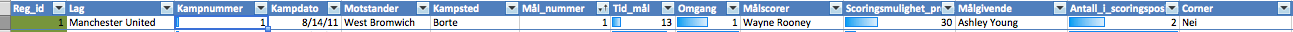
\includegraphics[width=1\textwidth]{images/general/prev_domain_model2.png}
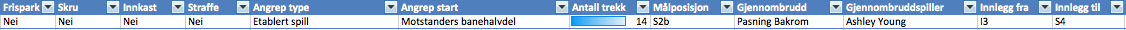
\includegraphics[width=1\textwidth]{images/general/prev_domain_model1.png}
\caption{A screen capture showing some data Tromsø IL captured in a previous analytic project.}
\label{fig:prevdomainmodel}
\end{figure}

From this we can define what the visioned system should capture from matches. The visioned system should capture from each match every successful attack that leads to an attempt on goal. Then from each attack you capture where the attack started, every pass including from/to zones, and type of attack. At last if there is a breaking point in the attack this should be captured. The breaking point of the attack should be stored with a breakthrough player and what type of breakthrough it was. Figure \ref{fig:different_break} illustrates the different breakthroughs we want to capture.

\begin{figure}[ht!]
\centering
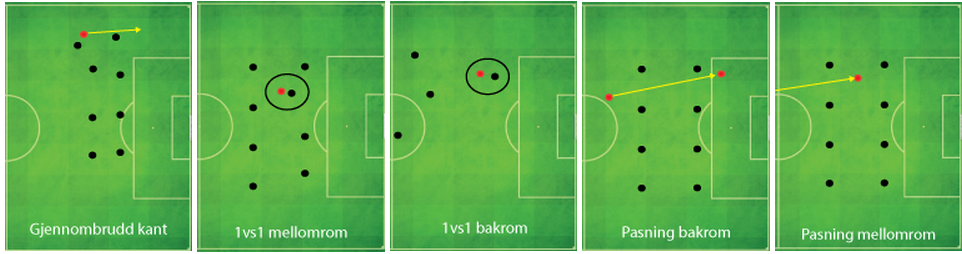
\includegraphics[width=1\textwidth]{images/general/different_breakthroughs.png}
\caption{Illustrations of different breakthroughs we want to capture.}
\label{fig:different_break}
\end{figure}

The visioned system needs a data store. The data should be stored in a database that has a rich query language for being able to support the large range of queries on the data. Good support for aggregate functions is crucial. The data will consist of text and integers.

Additionally an interface for input will be required. This interface should ensure that the input data is correct. For example when defining what type of attack the attack is, only the predefined options should be valid as input. 

Capturing every pass in successful attacks requires a positioning system. Here we suggest a more coarse grained dividing of the pitch than x,y co-ordinates like many systems use. We want to look at areas on the pitch The process of defining how to divide the pitch into zones took several rounds of discussion leading to several types. These are shown in figure \ref{fig:zones}.

\begin{figure}[ht!]
\centering
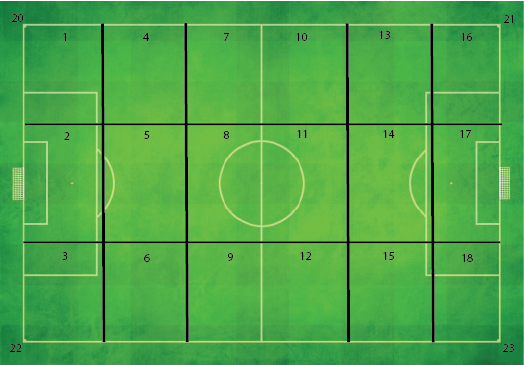
\includegraphics[width=100mm]{images/general/first_zones.png}
\caption{Dividing of pitch - the first suggestion had 18 zones}
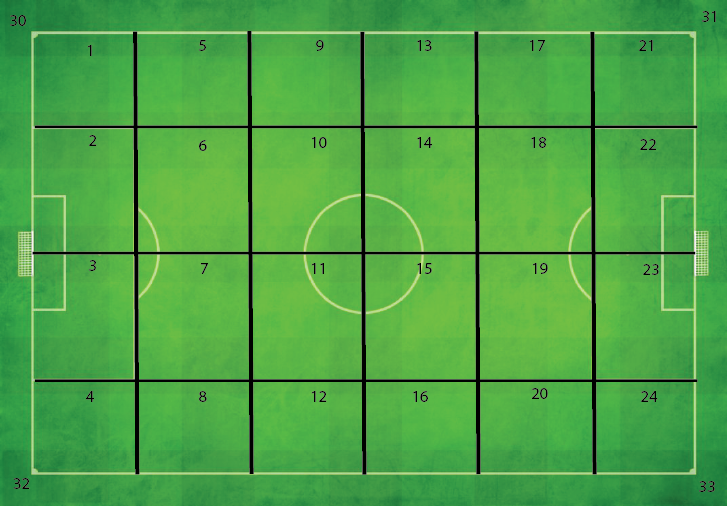
\includegraphics[width=100mm]{images/general/second_zones.png}
\caption{Dividing of pitch - the second suggestion had 24 zones}
\label{fig:zones}
\end{figure}


\section{Present}

The presentation of the data is an important aspect of the system. This will be where the end-users will spend their time. The presentation of data needs to be as simple as possible to understand. The coaching staff is no technical experts and the system is aimed for them to use. Therefor, the system will need to present statistics and other valuable information in a clean and understandable way. In the end it is the 11 players the coach selects that perform all the actions, but the coach sets the style of play and boundaries for players. The goal is to give the coach the opportunity to use the system, using both analytic illustrations and statistics, so he can better reach out to his players with his ideas. The better a coach can sell his ideas to the players the more they will believe in the philosophy, style of play and follow the game plan in games.

We purpose a web interface here, as it is accessible from many devices as long as you have an Internet connection and an up to date web browser. 

\Section{Summary}

To summarize we need a storage for persisting the data and run queries on, a back-end for transforming client requests to database operations, and an interface for capturing and presenting analytic information. Figure \ref{fig:conept_arch} shows the conceptual architecture. 

\begin{figure}[ht!]
\centering
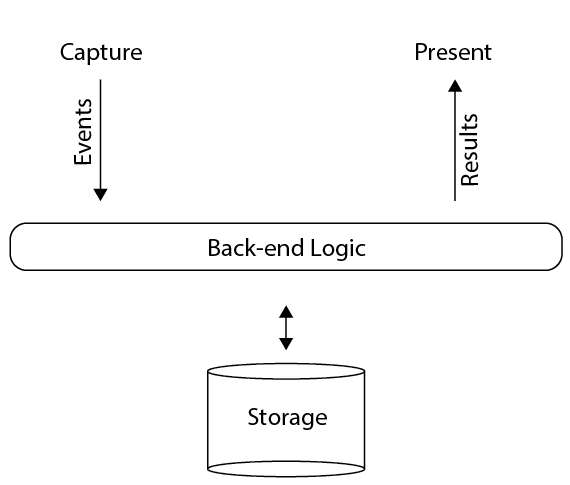
\includegraphics[width=150mm]{images/architecture/conceptual_architecture.png}
\caption{Conceptual architecture.}
\label{fig:conept_arch}
\end{figure}



